\documentclass[12pt]{article}
\usepackage{fullpage}
\usepackage{titlesec}
\usepackage{tikz}
\usepackage{amsfonts,amssymb}
\usepackage{amsmath}
\usepackage{comment}
\usetikzlibrary{automata, positioning}

\input ../libraries/mac.tex
\input ../libraries/mathmac.tex

\begin{document}
\pagestyle{plain}
\titleformat{\subsection}[runin]
  {\normalfont\large\bfseries}{\thesubsection}{1em}{}
\titleformat{\subsubsection}[runin]
  {\bfseries}{}{1em}{}

\title{Homework 6}
\author{Brooke Fugate, Michael O'Connor, Rohan Shah}
\date{}

\maketitle

\newpage
\section*{Problem B1}
\subsection*{(i)}
NFA $N_{C_G}$ for the grammer $G$:
\begin{center}
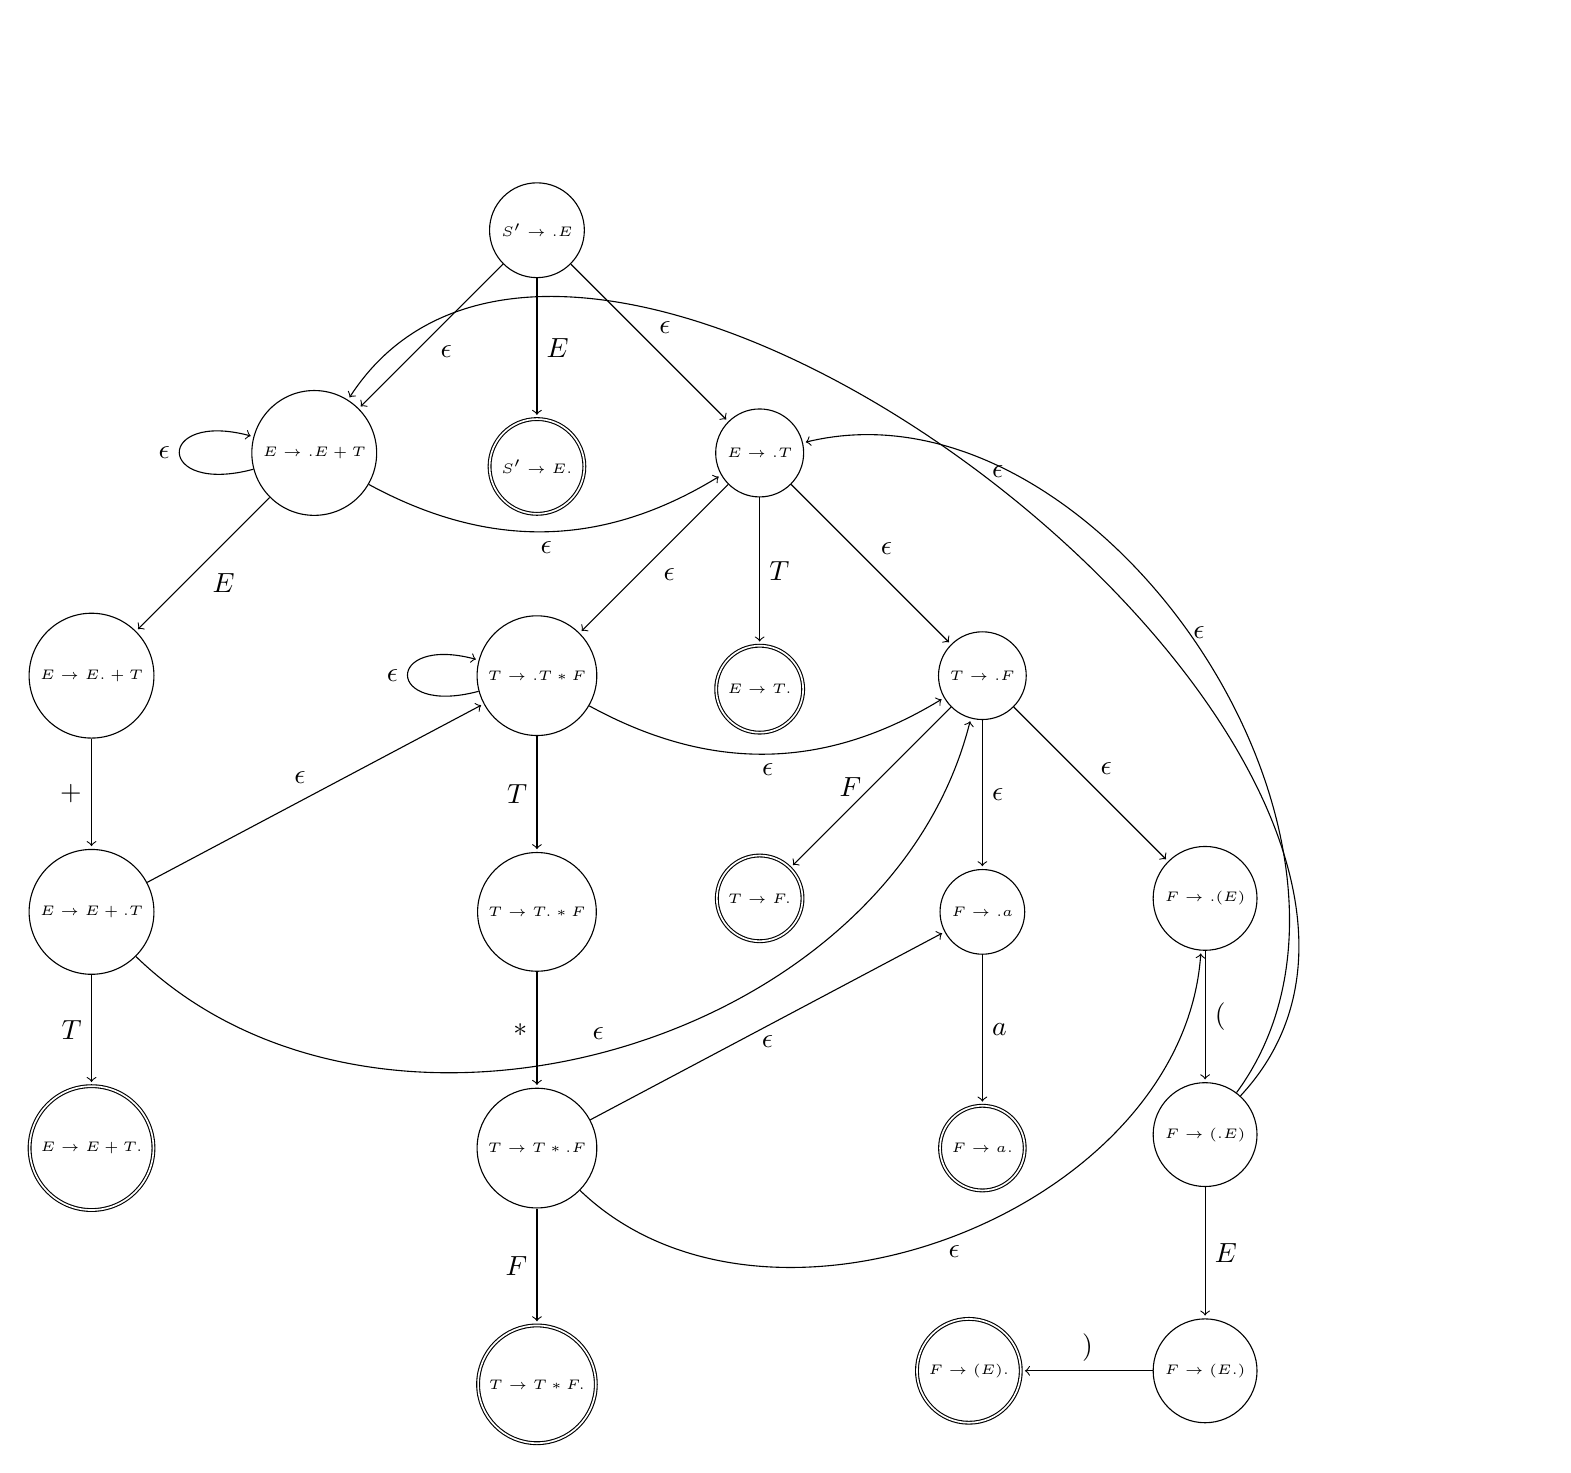
\begin{tikzpicture}[shorten >=1pt, node distance=3cm, on grid, auto]
  \node[state] (q0) {\tiny $S' \rightarrow .E$};
  \node[state, accepting] (q1) [below=of q0] {\tiny $S' \rightarrow E.$};
  \begin{scope}[node distance=4cm]
  \node[state] (q2) [below left=of q0] {\tiny $E \rightarrow .E+T$};
  \node[state] (q3) [below right=of q0] {\tiny $E \rightarrow .T$};
  \node[state] (q4) [below left=of q2] {\tiny $E \rightarrow E.+T$};
  \end{scope}
  \node[state, accepting] (q5) [below=of q3] {\tiny $E \rightarrow T.$};
  \begin{scope}[node distance=4cm]
  \node[state] (q6) [below left=of q3] {\tiny $T \rightarrow .T*F$};
  \node[state] (q7) [below right=of q3] {\tiny $T \rightarrow .F$};
  \end{scope}
  \node[state] (q8) [below=of q4] {\tiny $E \rightarrow E+.T$};
  \node[state] (q9) [below=of q6] {\tiny $T \rightarrow T.*F$};
  \node[state] (q12) [below=of q7] {\tiny $F \rightarrow .a$};
  \begin{scope}[node distance=4cm]
  \node[state, accepting] (q10) [below left=of q7] {\tiny $T \rightarrow F.$};
  \node[state] (q11) [below right=of q7] {\tiny $F \rightarrow .(E)$};
  \end{scope}
  \node[state, accepting] (q13) [below=of q8] {\tiny $E \rightarrow E+T.$};
  \node[state] (q14) [below=of q9] {\tiny $T \rightarrow T*.F$};
  \node[state] (q15) [below=of q11] {\tiny $F \rightarrow (.E)$};
  \node[state, accepting] (q16) [below=of q12] {\tiny $F \rightarrow a.$};
  \node[state, accepting] (q17) [below=of q14] {\tiny $T \rightarrow T*F.$};
  \node[state] (q18) [below=of q15] {\tiny $F \rightarrow (E.)$};
  \node[state, accepting] (q19) [left=of q18] {\tiny $F \rightarrow (E).$};

  \path[->]
  (q0) edge node {$E$} (q1)
  (q0) edge node {$\epsilon$} (q2)
  (q0) edge node {$\epsilon$} (q3)
  (q2) edge node {$E$} (q4)
  (q2) edge [loop left] node {$\epsilon$} (q2)
  (q2) edge [bend right] node [below] {$\epsilon$} (q3)
  (q3) edge node {$T$} (q5)
  (q3) edge node {$\epsilon$} (q6)
  (q3) edge node {$\epsilon$} (q7)
  (q4) edge node [left] {$+$} (q8)
  (q6) edge node [left] {$T$} (q9)
  (q6) edge [loop left] node {$\epsilon$} (q6)
  (q6) edge [bend right] node [below] {$\epsilon$} (q7)
  (q7) edge node [left] {$F$} (q10)
  (q7) edge node {$\epsilon$} (q11)
  (q7) edge node {$\epsilon$} (q12)
  (q8) edge node [left] {$T$} (q13)
  (q8) edge node {$\epsilon$} (q6)
  (q8) edge [bend right=60] node {$\epsilon$} (q7)
  (q9) edge node [left] {$*$} (q14)
  (q11) edge node {$($} (q15)
  (q12) edge node {$a$} (q16)
  (q14) edge node [left] {$F$} (q17)
  (q14) edge [bend right=65] node [below] {$\epsilon$} (q11)
  (q14) edge node [below] {$\epsilon$} (q12)
  (q15) edge node {$E$} (q18)
  (q15) edge [bend right=95] node [above] {$\epsilon$} (q2)
  (q15) edge [bend right=70] node [above] {$\epsilon$} (q3)
  (q18) edge node [above] {$)$} (q19)
  ;
\end{tikzpicture}
\end{center}

\newpage
\subsection*{(ii)}
DFA $D_{C_G}$ for the grammer $G$:
\newline
\begin{tikzpicture}[shorten >=1pt, node distance=3cm, on grid, auto]
  \node[state] (0) {0};
  \node[state] (4) [below=of 0] {4};
  \begin{scope}[node distance=2cm]
  \node[state, accepting] (3) [left=of 4] {3};
  \node[state, accepting] (1) [left=of 3] {1};
  \end{scope}
  \node[state, accepting] (5) [right=of 0] {5};
  \node[state] (6) [below=of 1] {6};
  \node[state] (8) [below=of 4] {8};
  \node[state, accepting] (2) [right=of 8] {2};
  \node[state] (7) [below=of 2] {7};
  \node[state, accepting] [below=of 6] (9) {9};
  \node[state, accepting] [right=of 7] (10) {10};
  \begin{scope}[node distance=2.5cm]
  \node[state, accepting] [below=of 8] (11) {11};
  \end{scope}

  \path[->]
  (0) edge node [above] {E} (1)
  (0) edge [bend left] node {T} (2)
  (0) edge node [left] {F} (3)
  (0) edge node [left] {(} (4)
  (0) edge node {a} (5)
  (1) edge node [left] {+} (6)
  (2) edge node {*} (7)
  (4) edge node [left] {E} (8)
  (4) edge node {T} (2)
  (4) edge node [above] {F} (3)
  (4) edge [loop right] node {(} (4)
  (4) edge node [below] {a} (5)
  (6) edge node [left] {T} (9)
  (6) edge node [above] {F} (3)
  (6) edge node [below] {(} (4)
  (6) edge [bend left=100] node {a} (5)
  (7) edge node {F} (10)
  (7) edge node {(} (4)
  (7) edge [bend right] node [right] {a} (5)
  (8) edge node [left] {)} (11)
  (8) edge node {+} (6)
  (9) edge [bend right] node [below] {*} (7)
  ;
\end{tikzpicture}

\newpage
\subsection*{(iii)} Let $G$ be a reduced context-free grammar where
$G = (V,\Sigma,P,S')$ and let $C_G$ be the set of characteristic strings of $G$
defined as:
$$C_G = \{\alpha\beta \in V^* \mid S' \underset{rm}{\Longrightarrow}^* \alpha Bv
\underset{rm}{\Longrightarrow} \alpha\beta v,\ \alpha,\beta \in V^*,\ v\in
\Sigma^*,\ B \rightarrow \beta \in P \}$$
Let $N_{C_G} = (Q,\Sigma,\delta,q_0,F)$ be the NFA constructed according to the
method described in Section 1 of the handout
\textit{A Survey of LR-Parsing Methods etc.}
\medskip\newline
\textbf{Claim:} For every rightmost derivation
$$A \overset{n}{\underset{rm}{\Longrightarrow}} \alpha Bv
\underset{rm}{\Longrightarrow}
\alpha\beta v \text{ implies } \delta^*((A \rightarrow \text{ "."}\zeta)
,\ \alpha\beta) = (B \rightarrow \beta\text{"."})$$
where $n\ge 0,\ v \in \Sigma^*$, $A,B\in N$, $\alpha,\beta\in V^*$,
$(A \rightarrow \text{ "."}\zeta)\in Q$, $(B \rightarrow \beta\text{"."})\in F$
and $A \rightarrow \zeta$ is the first production in the above rightmost
derivation.
\medskip\newline
\textbf{Proof:} By induction on the n.
\medskip\newline
\textbf{Base Case:} n = 0. So we have
$$A \underset{rm}{\Longrightarrow} \alpha\beta v \text{ and } A \rightarrow \zeta$$
therefore $A = B$, $\zeta = \beta$, and $\alpha, v = \epsilon$
so we need to prove that
$$\delta^*((B \rightarrow \text{"."}\beta),\ \beta) =
(B \rightarrow \beta\text{"."})$$
which is trivially true by the construction of $N_{C_G}$.
\medskip\newline
\textbf{Induction Case:} By the induction hypothesis we have
$$B_i \overset{n_2}{\underset{rm}{\Longrightarrow}} \alpha_i Bw_i
\underset{rm}{\Longrightarrow} \alpha_i \beta w_i \text{ implies }
\delta^*((B_i \rightarrow\text{"."}\zeta_i), \alpha_i \beta) =
(B \rightarrow \beta\text{"."})$$
where $n_2 < n$ and $B_i \rightarrow \zeta_i$ is the first production applied
in the rightmost derivation from $B_i$. We have that

$$A \underset{rm}{\Longrightarrow} \lambda B_{i}\rho
\overset{n_1}{\underset{rm}{\Longrightarrow}} \lambda B_{i}w
\overset{n_2}{\underset{rm}{\Longrightarrow}} \lambda \alpha _{i}Bw_{i}w
\underset{rm}{\Longrightarrow} \lambda \alpha _{i}\beta w_{i}w$$
where $w,w_i \in \Sigma^*$, $A,B,B_i \in  N$,
$\lambda, \rho, \alpha_i, \beta\in  V^*$,
$\rho \underset{rm}{\Longrightarrow}^* w$, and
$A \rightarrow \lambda B_{i}\rho$ is the first production in the above rightmost
derivation. By the construction of $N_{C_G}$ we have that
$$\delta^*((A \rightarrow \text{ "."}\lambda B_i \rho),\ \lambda) =
(A \rightarrow \lambda\text{ "."} B_i \rho)$$
$$\delta^*((A \rightarrow \lambda\text{ "."} B_i \rho),\ \epsilon) =
(B_i \rightarrow \text{ "."}\zeta_i)$$
and from the induction hypothesis we have that
$$\delta^*((B_i \rightarrow\text{"."}\zeta_i), \alpha_i \beta) =
(B \rightarrow \beta\text{"."})$$
so by the transitivity of $\delta^*$ we have that
$$\delta^*((A \rightarrow \text{ "."}\lambda B_i \rho),\ \lambda\alpha_i\beta) =
(B \rightarrow \beta\text{"."})$$
where in our claim $\alpha = \lambda\alpha_i$ and $v = w_iw$.
By the definition of $C_G$ we have that if $\alpha\beta \in C_G$ then there
is a rightmost derivation of the form
$$S' \underset{rm}{\Longrightarrow}^* \alpha Bv
\underset{rm}{\Longrightarrow} \alpha\beta v$$
Using the claim we just proved we have that
$$\delta^*((S' \rightarrow \text{"."}\zeta), \alpha\beta) =
(B \rightarrow \beta\text{"."})$$
where $(S' \rightarrow \text{"."}\zeta)$ is the start state and
$(B \rightarrow \beta\text{"."})$ is a final state by the construction
of $N_{C_G}$ which means that $\alpha\beta \in L(N_{C_G})$.
Therefore we have that $C_G \subseteq L(N_{C_G})$.
\medskip\newline
\textbf{Claim: } For any state $(A \rightarrow \text{ "."}\zeta) \in Q$,
$$\delta^*((A \rightarrow \text{ "."}\zeta),\ \gamma) =
(B \rightarrow \beta\text{"."}) \in F \text{ implies }
A \underset{rm}{\Longrightarrow}^* \alpha Bv \underset{rm}{\Longrightarrow}
\alpha \beta v$$
such that, the production applied in the first
rightmost derivation step is $A \rightarrow \zeta$, and $\gamma=\alpha\beta$.
\medskip\newline
\textbf{Proof: } By induction on the number of $\epsilon$-transitions in a
computation in $N_{C_G}$
\medskip\newline
\textbf{Base Case:} 0 $\epsilon$-transitions. Then by the construction of
$N_{C_G}$ if
$$\delta^*((A \rightarrow \text{ "."}\zeta),\ \gamma) =
(B \rightarrow \beta\text{"."})$$
then $\gamma = \zeta$  and the above computation is equivalent to
$$\delta^*((A \rightarrow \text{ "."}\zeta),\ \zeta) =
(A \rightarrow \zeta\text{ "."})$$
and the claim trivially holds where $A=B$, $\alpha, v =\epsilon$, $\beta=\zeta$
and the single production in the rightmost derivation is $A \rightarrow \zeta$.
\medskip\newline
\textbf{Induction Case:} $n$ $\epsilon$-transitions and where by the induction
hypothesis we have
$$\delta^*((B_i \rightarrow\text{"."}\zeta_i), \alpha_i \beta) =
(B \rightarrow \beta\text{"."}) \text{ implies }
B_i \underset{rm}{\Longrightarrow}^* \alpha_i Bw_i
\underset{rm}{\Longrightarrow} \alpha_i \beta w_i$$
where $B_i \rightarrow \zeta_i$ is the first production applied
in the rightmost derivation from $B_i$ and there are less than $n$
$\epsilon$-transitions in the computation. Since there a non-zero number of
$\epsilon$-transitions, $\zeta$ is of the form $\lambda B_i\rho$
and $\gamma$ is of the form $\lambda \alpha_i \beta$ so we also have that
$$\delta^*((A \rightarrow \text{ "."}\lambda B_i\rho),\ \lambda\alpha_i\beta) =
(B \rightarrow \beta\text{"."})$$
By the transitivity of $\delta^*$ we have the following decomposition of the
above computation
$$\delta^*((A\rightarrow \text{"."}\lambda B_i\rho),\ \lambda) =
(A\rightarrow \lambda\text{"."}B_i\rho)$$
$$\delta^*((A\rightarrow \lambda\text{"."}B_i\rho),\ \epsilon) =
(B_i \rightarrow \text{"."}\zeta_i)$$
$$\delta^*((B_i \rightarrow \text{"."}\zeta_i),\ \alpha_i\beta) =
(B\rightarrow \beta\text{"."})$$
By construction of $N_{C_G}$ and the fact that there are no useless terminals in
$G$ we have that
$$A \underset{rm}{\Longrightarrow}^* \lambda B_i \rho
\underset{rm}{\Longrightarrow}^* \lambda B_i w$$
and by the induction hypothesis we have that
$$B_i \underset{rm}{\Longrightarrow}^* \alpha_i Bw_i
\underset{rm}{\Longrightarrow} \alpha_i \beta w_i$$
so we have that
$$A \underset{rm}{\Longrightarrow}^* \lambda B_i w
\underset{rm}{\Longrightarrow} \lambda\alpha_i \beta w_i w$$
and therefore our claim holds where $\alpha = \lambda\alpha_i$, $v=w_iw$.
By definition, if $\alpha\beta \in N_{C_G}$ then there exists some computation
of the form
$$\delta^*((S'\rightarrow \text{"."}\zeta),\alpha\beta) =
(B\rightarrow \beta\text{"."})$$
and by applying our claim have
$$ S' \underset{rm}{\Longrightarrow}^* \alpha Bv
\underset{rm}{\Longrightarrow} \alpha\beta v$$
So, by definition, $\alpha\beta \in C_G$ which implies that
$L(N_{C_G}) \subseteq C_G$.
\medskip\newline
Since we have proven that $C_G \subseteq L(N_{C_G})$
and that $L(N_{C_G}) \subseteq C_G$ it follows that $C_G = L(N_{C_G})$.

\section*{Problem B2}
\subsection*{i}
Proof that $v_j = f(u_j, \ptb{x})$ by induction on $|u_j|$: \newline
$|u_j| = 0 \rightarrow u_j = \epsilon \rightarrow f(\epsilon, \ptb{x}) = g(\ptb{x}) = v_0$\newline
$|u_j| \ge 1 \rightarrow f(u_j, \ptb{x}) = f(u_{j-1}a_{i_j}, \ptb{x}) = h_j(u_{j-1}, f(u_{j-1}, \ptb{x}), \ptb{x}) = h_j(u_{j-1}, v_{j-1}, \ptb{x}) = v_j$

\subsection*{ii}
We need to make a sketch of a RAM  program here that I just havent done yet. Initial sketch:\newline
assume we have 2 new functions suphead and revhead which work as follows: $$suphead(ya_j) = y : suphead(\epsilon) = \epsilon)$$ $$revhead(ya_j) = a_j : revhead(\epsilon) = epsilon$$ and that there exist RAM functions $g , h$, where $h$ is expecting input to be in $R3$.  Also let us assume that $R1$ is initialized with $u_j$ and $R2$ is initialized with $\ptb{x}$
$$R3 \leftarrow R1$$
$$R4 \leftarrow R3$$
$$suphead R3$$
$$revhead R4$$
$$R4,  \text{ }  jmp_{a_1},  \text{ }  N1b$$
$$R4,  \text{ }  jmp_{a_2},  \text{ }  N2b$$
$$...$$
$$R4,  \text{ }  jmp_{a_k},  \text{ }  Nkb$$
$$jmp \text{ } N(k+1)b$$
$$N1,  \text{ } h$$
$$N2,  \text{ } h$$
$$...$$
$$Nk,  \text{ } h$$
$$N(k+1), \text{ }  g$$
$$R1 \leftarrow R3$$

\section*{Problem B3}
We can prove that the function, $\mapdef{f}{\Sigma^*}{\Sigma^*}$, is primitive recursive by showing it as a primitive recursive function. \newline
$$f(\epsilon) = \epsilon $$
$$f(w) = a_1^{|w|} \rightarrow f(w) = f(ua_i) \rightarrow f(ua_i) = h_1(u, f(u)) \rightarrow h_1(u, f(u))= S_1 o P^2_2(u, f(u)) = f(w)$$

\section*{Problem B4}
\subsection*{A(0, x)} 
$$A(0, x) = x + 1$$
\subsection*{A(1, x)}
$$A(1, 0) = A(0, 1) = 2$$
$$A(1, x + 1) = A(0, A(1, x)) = A(0, x + 2) = x + 3 = (x + 1) +2$$
\subsection*{A(2, x)} 
$$A(2, 0) = A(1, 1) = A(0, A(1, 0) = A(0, 2) = 3$$
$$A(2, x + 1) = A(1, A(2, x)) = A(1, 2x + 3) = (2x + 3) +2 = 2x + 5 = 2(x + 1) + 3$$
\subsection*{A(3, x)} 
$$A(3, 0) = A(2, 1) = A(1, A(2, 0) = A(1, 3) = 5$$
$$A(3, x + 1) = A(2, A(3, x)) = A(2, 2^{x + 3} - 3) = 2*(2^{x+3} - 3)  + 3 = 2^{x + 1 + 3} - 3$$
\subsection*{A(4, x)} 
$$A(4, 0) = A(3, 1) = 2^{1 + 3} - 3 = 2^4 -3 = 13$$
$$A(4, x + 1) = A(3, A(4, x)) = A(3,  \supexpo{2}{2}{x + 3}\> - 3) = (2^{\supexpo{2}{2}{x + 3}\>} - 3 = \supexpo{2}{2}{x + 1 + 3}\> - 3$$

\section*{Problem B5}
\subsection*{a}
Prove that telling if a partial recursive function is a constant function is undecidable.  The property that a partially recursive function is a constant function, denotated P, is decidable iff the set $P_C = \{P(a)|a \in C and P(a)\}$ is recursive, where C is the set of partially recursive functions that are constant functions. By the Rice Theorem, the set $P_C$ is non-recursive unless C is trivial.  For C to be trivial it must either be the empty set or be the set of all recursive functions. The function $f(x)=0$ is partially recursive and is a constant set, so C is not empty.  The successor function is an example of a partially recursive function that is not constant, so C is not the set of all partially recursive functions.  So we know that C is not trivial, therefore $P_C$ is not recursive and P must be undecidable. 
\subsection*{b} 
Prove that the property of two partial recursive functions being identical is undecidable.  We will reduce the set $P_B = \{x,y \in \mathbb{N} | \varphi_x = \varphi_y\}$ to the set $P_C = \{x \in \mathbb{N} | \varphi_x = \varphi_a \}$.  Since we know C is undecidable from part c) reducing C to B will show that B is undecidable. To show that C is reducable to B  we need to show that there is a function from $f : C \rightarrow B$.  $x \in C \text{ iff } f(x) \in B$ so if $f(x) = < x , a >$ then C is reducable to B, therefore B is undecidable.
\subsection*{c} 
Prove that the property of a partial recursive function $\varphi_x$ is equal to a given partial recursive function $\varphi_a$ is not decidable.  As in (a), we must show that the set $P_C = \{x \in \mathbb{N} | \varphi_x = \varphi_a \}$ to is non-trivial.  The set is not empty because $\varphi_a = \varphi_a$ and the set is not the set of all partially recursive functions because $S (\varphi_a(x)) \neq \varphi_a(x)$, so the set is not trivial and is therefore non-recursive, and the property on partially recursive functions is undecidable.  
\subsection*{d}
Prove that telling if a partial recursive function diverges for all input is not decidable.  As in (c), we must show that the set $P_C = \{x \in \mathbb{N} | \varphi_x \text{is undecidable for all inputs} \}$ is non-trivial.  The set is not empty because we can define a function $\forall x \mid \varphi_a(x) = undecidable$ and the set is not the set of all partially recursive functions because the successor function is not undecidable on all inputs, so the set is not trivial and is therefore non-recursive, and the property on partially recursive functions is undecidable.  

\section*{Problem B6}

For any Grammar $G$ we can build a turing machine $T_G$ such that $L(G) = L(T_G)$.  If we have a turing machine $T_G$ it is partially recursive so if we an index on the partially recursive functions we can make a characteristic $P_C = \{x \in \mathbb{N} | \varphi_x \text{ generates a regular and CF language} \}$.  $P_C$ is not empty because the grammar $G = S \rightarrow ab$ produces both a context free grammar and a regular language and can be turned into a partially recursive function, from above.  $P_C$ is not all the partially recursive functions because the a grammar G:$$G = S \rightarrow aAb$$ $$A \rightarrow aAb | ab | \epsilon$$  This produces the langauges: $a^nb^n$ is context free but not a regular language.  So this is undecidable.

\section*{Problem B7}
\subsection*{i}
To show that the tiling problem with a single initial tile is NEXP-complete, we must show that the tiling problem $\in$ NEXP and the tiling problem is NEXP-hard. To show that it is $\in$ NEXP, we must prove there is an exponentially bounded nondeterministic Turing machine that accepts the tiling problem with a single initial tile. The size of the rectangular grid is $2s^2$, which is exponential in the length of the input, $log_2s+C+1$, so we need to check an exponential in the length of the input number of tiles to see if our solution is correct, and we can do this with an exponentially bounded nondeterministic Turing machine.
To show that the tiling problem is NEXP-hard, we must show that there is a polynomial reduction from every language $L_1 \in NEXP$ to L. Similarly to how the origional tiling problem from the course slides was shown to be NP-hard, we can show that this version is NEXP-hard.  Let $L \subseteq \Sigma^*$ be any language in NP and let u be any string in $\Sigma^*$. Assume that L is accepted in exponential time.  Construct an instance of the tiling probem, similarly to in the course slides, so that $u \in L$ iff the tiling problem has a solution.

\subsection*{ii} 
We proceed similarly to the proof in the course slides, except we remove tiles of type 5, but still keep the blank tiles.  We then show that if we can decide that a tiling exists, then we can show that the Turing machine is not divergent. Because we know the problem of deciding whether a Turing machine diverges in undecibable, this version of the tiling problem is also undecidable. 

\section*{Problem B8}
\subsection*{i}
It is clear that the 0-1 integer programming problem has the same complexity as multiplying a matrix by a vector if you can guess the solution, so it is in NP.

\subsection*{ii}
We start by allowing $x_{mnt} \in \{0,1\}$.  We see that to express the fact that every position is tiled by a
single tile, we use the equation
\[
\sum_{t\in \s{T}} x_{m n t} = 1,
\]
for all $m, n$ with $1 \leq m \leq 2 s$ and $1 \leq n \leq s$.
Then, we set the horizontal constraints 
\[
x_{mnt} + \sum_{t'} x_{(m+1) n t'} \le 1
\] 
for all $(t,t') \in \s{T} x \s{T} - H$ and we set the vertical constriants 
\[
x_{mnt} + \sum_{t'} x_{m (n+1) t'} \le 1
\] 
for all $(t,t') \in \s{T} x \s{T} - V$.  We let $\sigma_0$ be the perscribed bottom row, and we have $x_{m1\sigma_0 (m)} = 1$. To change the inequalities to equalities, we add slack variables so that the functions become: for the horizontal constraints
\[
x_{mnt} + \sum_{t'} x_{(m+1) n t'} + x'_{mnt} = 1
\]
for all $(t,t') \in \s{T} x \s{T} - H$ and for the vertical constriants
\[
x_{mnt} + \sum_{t'} x_{m (n+1) t'} + y_{mnt}  = 1
\]
for all $(t,t') \in \s{T} x \s{T} - V$ and $x_{m1\sigma_0 (m)} + z_{mnt} = 1$.
Using these equations we relate the tiling problem to a system of linear equations.  It is clear that a solution to the system of linear equations is found iff the tiling problem has a solution. We have shown a polynomial-time reduction from the bounded-tiling problem and therefore it is shown that the 0-1 integer programming problem is NP-Complete.  

\subsection*{iii}
It is clear from the proof of part ii that the restricted 0-1 integer programming problem in which the coefficients of A are 0 or 1 and all entries in b are equal to 1 is also NP-complete.

\end{document}
